\documentclass[12pt]{report}

\usepackage{listings}
\usepackage{xcolor}
\usepackage{graphicx}
\usepackage{amsmath}
\usepackage{hyperref}
\usepackage{geometry}
\usepackage{subfig}
\usepackage{float}
\usepackage{pgfplots}

\geometry{a4paper, margin=1in}
\pgfplotsset{compat=1.18}

\lstdefinestyle{bashstyle}{
    language=bash,
    basicstyle=\ttfamily\small,
    backgroundcolor=\color{black!5},
    frame=single,
    keywordstyle=\color{blue}\bfseries,
    commentstyle=\color{gray}\itshape,
    stringstyle=\color{green!50!black},
    morekeywords={vlog,vsim,run},
    alsoletter={-},
    breaklines=true,
    showstringspaces=false,
    columns=fullflexible
}

\lstdefinestyle{svstyle}{
    language=Verilog,
    basicstyle=\ttfamily\small,
    backgroundcolor=\color{black!5},
    frame=single,
    keywordstyle=\color{blue}\bfseries,
    commentstyle=\color{gray}\itshape,
    stringstyle=\color{green!50!black},
    morekeywords={logic, always_comb, always_ff, assign, begin, end, module, endmodule, if, else, for, return, typedef, enum, int, task, endtask, function, endfunction},
    breaklines=true,
    showstringspaces=false,
    columns=fullflexible
}

\begin{document}

\title{\textbf{Low-Level HW Digital Systems II} \newline Assignment Report}
\author{\textbf{Savvas Tzanetis} \\ 10889}
\maketitle

\tableofcontents
\chapter{Introduction}
This report documents the design and verification of a single precision, 32-bit floating point adder based on IEEE-754. This project was created as an assignment in the \textbf{Low-Level HW Digital Systems II} class of the Aristotle University's Electrical and Computer Engineering department. The code for this project is available at this \textcolor{blue}{\href{https://github.com/stzanetis/FP32Adder}{GitHub repository}} page. \\

\noindent The adder is implemented using the \textit{SystemVerilog} language, using a testbench as well as \textit{SystemVerilog Assertions}, in order to verify the correct functionality of the design. More specifically, the design is in compliance with the IEEE Level 0 standard, meaning denormal inputs are treated as \textit{±zero} and \textit{NaN} inputs are treated as \textit{±infinity}. \\

\noindent The main module of the design is \lstinline{fp_adder.sv}, which is wrapped by \lstinline{fp_adder_top}, and holds the input and output registers. The main module instantiates six sub-modules in a seven-stage pipeline:

\begin{itemize}
    \item Sign Calculation
    \item Exponent Calculation
    \item Mantissa Addition and Alignment
    \item Truncation and Normalization
    \item Rounding
    \item Post-round Normalization
    \item Exception Handling
\end{itemize}

\noindent with sign calculation and post-round normalization performed inline.

\chapter{Circuit Design}

\section{Sign Calculation}
In the first stage of the adder, the sign of the result is calculated. This is computed combinationally inside the main module by comparing the magnitudes of the two operands as seen in the following code.

\hspace{10pt}

\begin{lstlisting}[style=svstyle]
sign = (a[31] == b[31]) ? a[31] : ((a[30:0] > b[30:0]) ? a[31] : b[31]);
\end{lstlisting}

\hspace{10pt}

\noindent If the signs of \textit{a} and \textit{b} are equal the resulting sign will be the same as either operand. Alternatively, the sign is taken from the operand with the greater unsigned magnitude. As noted in the coursework's requirements, in most adders another input signal functioning as the operand should used to define the type of operation, but for simplicity, in this design we only consider that subtraction is done when the two operands have different 
signs.

\section{Exponent Calculation Module}
In the next stage of the adder, the difference between the exponents of the two floating numbers is calculated. In more detail, the exponent calculation module, takes the two 8-bit biased exponents extracted from \lstinline{a[30:23]} and \lstinline{b[30:23]} as inputs and produces the following outputs:

\begin{itemize}
    \item \textbf{\lstinline{max_exp}:} The larger of the two exponents, serving as the starting exponent of the result before any normalization adjustments.
    \item \textbf{\lstinline{exp_diff}:} The absolute difference between the two exponents.
    \item \textbf{\lstinline{sign_exp_diff}:} A flag that is set to 1 when \lstinline{exp_a > exp_b}. This is later passed to the mantissa calculation module to indicate which operand is the smaller one in order to perform the necessary right-shift during alignment.
\end{itemize}

\newpage
\noindent The following code shows how this process was implemented:

\hspace{10pt}

\begin{lstlisting}[style=svstyle]
assign sign_exp_diff = (exp_a > exp_b);
assign max_exp       = sign_exp_diff ? exp_a : exp_b;
assign exp_diff      = sign_exp_diff ? ({1'b0, exp_a} - {1'b0, exp_b}) : ({1'b0, exp_b} - {1'b0, exp_a});
\end{lstlisting}

\section{Mantissa Calculation Module} \label{mantissa-calc-module}
The mantissa calculation module is responsible for two steps in the adder's implementation, the mantissa alignment, as well as the addition and subtraction on the two operands mantissas. The output of this module is a 27-bit mantissa resulted from the aforementioned operations.

\subsection{Alignment}
Both mantissas arrive inside the module as 24-bit values, composed of the 23 fraction bits and an implicit 1 that is added in the main module. During the alignment process, the operand with the smaller exponent is right-shifted by $N$ positions, where $N$ is equal to the difference between the two operands, calculated during the previous step. This shifting process has a critical design concern that is taken into consideration in this design, this operation may cause the loss of information (bits), affecting the adder's rounding accuracy. To combat this, the smaller of the two mantissas is placed in the upper half of a 49-bit intermediate signal, during the operation:

\hspace{10pt}

\begin{lstlisting}[style=svstyle]
logic [48:0] shift_in;
logic [48:0] shifted_val;
assign shift_in = {mant_smaller, 25'b0};
assign shifted_val = shift_in >> d;
\end{lstlisting}

\hspace{10pt}

\noindent After the shift three extra precision bits are extracted from the lower portion of of the shifted value, the \textit{Guard} bit, the \textit{Round} bit as well as the \textit{Sticky} bit. These three bits, called GRS bits, are essential for correct rounding in later stages. \\

\noindent Finally, the aligned smaller mantissa consists of the aforementioned shifted value, in addition to the GRS bits and is 27-bit long. The larger mantissa is similarly widened to 27 bits by being padded with three zeros at the LSB end.

\subsection{Addition}
After alignment, all that is left is the addition, or subtraction in the case of different signs, of the two mantissas. Since  the sign has already been resolved in the first stage, subtraction always removes the smaller mantissa from the larger one, guaranteeing a positive result.
 
\section{Normalization Module}
The IEEE-754 standard requires that the mantissa of the resulting floating point number is in a normalized form, and more specifically that exactly one non-zero bit to be added to the left of the binary point. The normalization module, handles this exact logic.

\noindent While implementing this logic, the case where a result is $< 1$ must be handled by being left-shifted. For this, a helper module was implemented, the \textit{Leading Zero Counter}, which is responsible for outputing a 5-bit count of leading zeroes from the 28-bit input mantissa from \ref{mantissa-calc-module}, by scanning from the most significant bit downwards using a loop.

\noindent The normalization itself is later handled with the following four cases:
\begin{itemize}
    \item \textbf{Result is Zero}: Occurring after an exact cancellation of the equal, with opposite sign, operands
    \item \textbf{Bit 27 is Set}: Where the mantissa must be right-shifted by one position and the exponent incremented by one
    \item \textbf{Bit 26 is Set, Bit 27 is Clear}: Where the mantissa is already in the correct normalized form and can be passed through unchanged
    \item \textbf{Bits 26 and 27 are Clear}: Where a left shift is needed to push the leading 1 into bit 26. The required shift amount is the number of leading zeroes calculated in the LZC module, minus 1, since LZC counts from bit 27 while the target position is bit 26. 
\end{itemize}

\noindent During the operation of the last case, exponent underflow must be avoided. This is guarded explicitly:

\hspace{10pt}

\begin{lstlisting}[style=svstyle]
if ({1'b0, max_exp} > {4'b0, shift_amt})
    norm_exp = {1'b0, max_exp}- {4'b0, shift_amt};
else
    norm_exp = 9'd0;
\end{lstlisting}

\section{Rounding Module}
The rounding module accepts the 26-bit normalized mantissa, the 3-bit rounding mode, and the calculated sign bit, producing a 25-bit rounded mantissa and an inexact flag. This is achieved using the \lstinline{round_pkg} package which defines the rounding mode enumerations. The five supported rounding modes are listed below in Table \ref{fig:rounding_modes}:

\begin{figure}[ht]
    \centering
    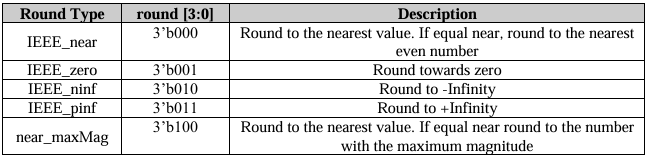
\includegraphics[width=0.9\linewidth]{assets/rounding_modes.png}
    \caption{Rounding Types}
    \label{fig:rounding_modes}
\end{figure}

\section{Post-round Normalization}
After all of the above steps are taken, a post-rounding normalization occurs, which is implemented inside the adder's main module. This prevents the rare case where a during the rounding process, the mantissa incrementation can cause an overflow. In such a case, this is fixed with a single right-shift, in addition to incrementing the exponent by $1$. \\

\noindent During this stage, the case of either an overflow or underflow occurring in the final exponent is detected. The intermediate result \lstinline{z_calc} is then assembled.

\section{Exception Module}
The final stage, the exception handling stage, is implemented in a separate module as described by the coursework.  This module is responsible for detecting cases such as the inputs or intermediate results don't follow the regular addition path, producing the correct result and status flags.

\noindent In more detail, the following special cases are handled:
\begin{itemize}
    \item \textbf{Zero + Zero:} Returns $+/-Zero$ with sign determined by the rounding mode
    \item \textbf{Infinity cases:} $+Inf + Normal = +Inf, -Inf + Normal = −Inf, +/-Inf + +/-Inf$ returns $+/-Inf$ or sets $NaN$ flag if signs differ.
    \item \textbf{Invalid operation:} $+Inf + (−Inf) = NaN$ (sets the \lstinline{nan_f} flag).
    \item \textbf{Overflow:} When the exponent exceeds the representable range, the result is set to $+/-Inf$ (or maxNormal depending on rounding mode), and the \lstinline{huge_f} flag is set.
    \item \textbf{Underflow:} When the exponent underflows, the result is set to $+/-Zero$ (or minNormal depending on rounding mode), and the \lstinline{tiny_f} flag is set.
\end{itemize}


\chapter{Verification}
\section{Testbench}
The testbench is written based on the provided \lstinline{tb_adder.sv} file and initiates the included \lstinline{fp_adder_top} wrapper alongside the included reference \textit{HardFloat} library, used for validating the results of the implemented adder. In more detail regarding the included reference library, \textit{HardFloat} internally uses a 33-bit recoded format for single precision, meaning that in order for the results to be correctly validated, the testbench uses the \lstinline{fNToRecFN} module to convert any inputs to this format, and later converts them back to a standard 32-bit IEEE format using the \lstinline{recFNToFN} module.

\subsection{Random Tests}
\lstinline{$urandom()} drives a and b with fresh 32-bit random values every cycle. The testbench only prints output when a mismatch is detected between \lstinline{result} and \lstinline{results_ref}, keeping the transcript readable for large numbers of tests. Random testing is effective at catching errors in the main arithmetic data path but is less suited to exercising rare special-value combinations, which is why the second phase is also required.

\hspace{10pt}

\begin{lstlisting}[style=svstyle]
for (int i = 0; i < 1000; i++) begin
    @(negedge clk);
    a = $urandom();
    b = $urandom();
    round = 3'b000;
end
\end{lstlisting}

\subsection{Corner Case Tests}
A dedicated function maps each value of a corner type enumerated type to a specific 32-bit IEEE bit-pattern. The ten corner cases selected for each of a and b are:
\begin{itemize}
\item Positive and negative $NaN$ (random non-zero mantissa, exponent all-ones)
\item Positive infinity and negative infinity
\item One random positive normal and one random negative normal
\item One random positive denormal and one random negative denormal
\item Positive zero and negative zero
\end{itemize}

\noindent All 100 combinations are tested sequentially against the reference, using the default rounding mode (round to nearest, tie to even). To accurately mirror the requirements, an array of exactly 10 values is generated once, and the 10x10 combinations are tested using those fixed values:

\hspace{10pt}

\begin{lstlisting}[style=svstyle]
for (int k = 0; k < 10; k++) begin
    corner_vals[k] = get_corner(corner_type_t'(k));
end

for (int i = 0; i < 10; i++) begin
    for (int j = 0; j < 10; j++) begin
        @(negedge clk);
        a = corner_vals[i];
        b = corner_vals[j];
        round = 3'b000;
    end
end
\end{lstlisting}

\section{Assertions}
Two assertion modules are binded to the wrapper module, keeping the assertion logic cleanly separated from both the DUT and the testbench.

\subsection{Immediate Assertions}
The \lstinline{test_status_bits} module checks in a combinational block that physically contradictory status flag combinations are never simultaneously enabled. In more detail, the checked illegal combinations are:

\begin{itemize}
\item \lstinline{zero_f} with any of: \lstinline{inf_f}, \lstinline{nan_f}, \lstinline{tiny_f}, \lstinline{huge_f}
\item \lstinline{inf_f} with any of: \lstinline{nan_f}, \lstinline{tiny_f}, \lstinline{huge_f}, \lstinline{zero_f}
\item \lstinline{nan_f} with any of: \lstinline{tiny_f}, \lstinline{huge_f}, \lstinline{inexact_f}
\item \lstinline{tiny_f} with \lstinline{huge_f}
\end{itemize}

\noindent Each violated assertion emits a descriptive error message identifying the specific conflicting pair.

\subsection{Concurrent Assertions}
Four property/assert pairs check structural relationships between the status flags and the output at every positive clock edge. Specifically:

\begin{itemize}
\item \textbf{\lstinline{p_zero}}: If \lstinline{zero_f} is set then all exponent bits of \lstinline{z} must be zero
\item \textbf{\lstinline{p_inf}}: If \lstinline{inf_f} is set then all exponent bits of \lstinline{z} must be ones
\item \textbf{\lstinline{p_nan}}: If \lstinline{nan_f} is set then two cycles earlier (matching the pipeline depth) both \textsc{a[30:23]} and \textsc{b[30:23]} must have been \textsc{FF} and the two sign bits must have differed
\item \textbf{\lstinline{p_huge}}: If \lstinline{huge_f} is set then the exponent of \lstinline{z} must be either \textsc{FF} or \textsc{FE} with the mantissa equal to all ones,  which is the \textit{MaxNormal} representation
\end{itemize}

\section{Simulation Results}
The simulations of this implementation were run using the Intel Questa simulation program. The code compilation as well as the simulation can be executed by running the following commands in the program's terminal:

\hspace{10pt}

\begin{lstlisting}[style=bashstyle]
vlog -sv round_pkg.sv
vlog -sv exponent_calc.sv mantissa_calc.sv lzc.sv norm_adder.sv
vlog -sv round_adder.sv exception_adder.sv fp_adder.sv
vlog -sv hardfloat/*.v
vlog -sv test_status.sv
vlog -sv tb_adder.sv
\end{lstlisting}

\hspace{10pt}

\noindent All tests and assertions passed successfully without producing any errors, as can be seen in figure \ref{fig:results} below:

\begin{figure}[ht]
    \centering
    \fbox{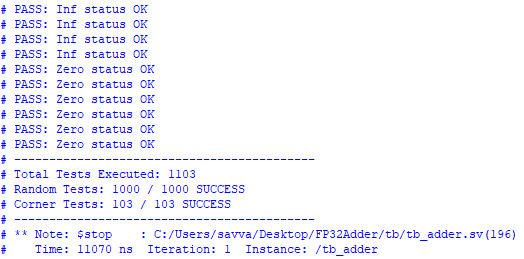
\includegraphics[width=0.7\linewidth]{assets/results.png}}
    \caption{Simulation Results}
    \label{fig:results}
\end{figure}

Additionally the waveforms of basic signals like operands a and b as well as the result and status can be seen in figure \ref{fig:waveform}.

\begin{figure}
    \centering
    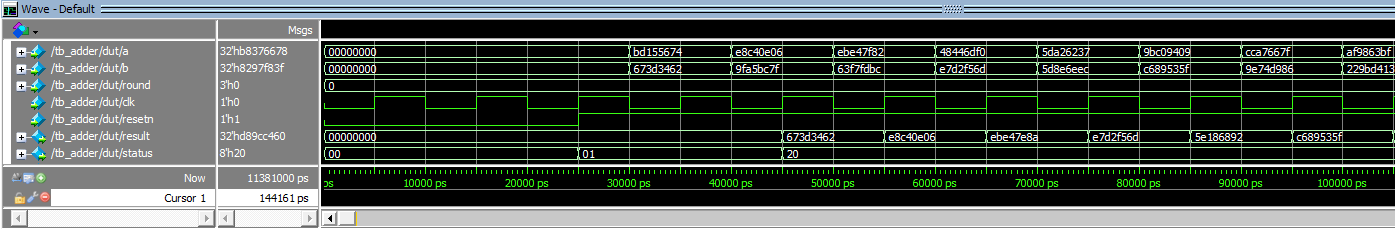
\includegraphics[width=0.9\linewidth]{assets/waveform.png}
    \caption{Waveform}
    \label{fig:waveform}
\end{figure}

\end{document}